\documentclass{article} %[a4paper, 10pt, french]

\usepackage[french]{babel}
\usepackage[utf8]{inputenc}
\usepackage[T1]{fontenc}
\usepackage{amsmath,amsfonts,amssymb,mathrsfs}
\frenchbsetup{StandardLists=true}
\usepackage{geometry}
\usepackage{lmodern} %pas pixelisé
\usepackage{engrec,titlesec,lipsum,xcolor}
\usepackage{fancybox}
\usepackage[skins, most]{tcolorbox}
\usepackage[bookmarks={true},bookmarksopen={true}, hidelinks, pdftitle={APP - Fil rouge}, pdfauthor={APProximatif}, pdfsubject={Arbres équilibres AVL}]{hyperref}
\usepackage{setspace}
\usepackage{mathabx}
\usepackage{multicol}
\usepackage{enumitem}
\usepackage{array,multirow,makecell}
\usepackage{titlesec}
\usepackage{multirow}
\usepackage{hyperref}
\usepackage{listings}
\usepackage{graphicx}
\usepackage{caption}
\usepackage{subcaption}
\usepackage{float}

\AddThinSpaceBeforeFootnotes
\FrenchFootnotes
\geometry{hmargin=1.2cm, top=1.2cm, bottom = 1.5cm}
\definecolor{vert}{rgb}{0,0.69,0.31}
\definecolor{bleue}{rgb}{0,0.31,0.69} 
\definecolor{violet}{rgb}{0.38,0.18,055} % 97, 45, 140     244, 208, 63
\definecolor{jaune}{rgb}{0.96, 0.85, 0.23}


\definecolor{darkWhite}{rgb}{0.94,0.94,0.94}
\definecolor{vert}{rgb}{0,0.69,0.31}
\definecolor{rose}{rgb}{1,0.08,0.58}% rgb(255,20,147)
\definecolor{rouge}{rgb}{0.78,0.12,0.08}
\definecolor{bleue}{rgb}{0,0.31,0.69}
\definecolor{gris}{rgb}{0.4,0.4,0.4}
\definecolor{marron}{rgb}{0.4,0.2,0}
\definecolor{darkWhite}{rgb}{0.94,0.94,0.94}

\newtcolorbox{titre}[1][]{enhanced, drop fuzzy shadow southwest, arc=4mm, outer arc=1mm, colback=red!5!white,colframe=red!75!black, boxrule=3pt, center, halign = center, left=1mm, right=1mm,  width = 7.7cm }



\renewcommand*{\lstlistlistingname}{Code Listings}
\renewcommand*{\lstlistingname}{Code Listing}
\definecolor{gray}{gray}{0.5}
\colorlet{commentcolour}{green!50!black}
\colorlet{stringcolour}{red!60!black}
\colorlet{keywordcolour}{magenta!90!black}
\colorlet{exceptioncolour}{yellow!50!red}
\colorlet{commandcolour}{blue!60!black}
\colorlet{numpycolour}{blue!60!green}
\colorlet{literatecolour}{magenta!90!black}
\colorlet{promptcolour}{green!50!black}
\colorlet{specmethodcolour}{violet}


\newcommand*{\framemargin}{3ex}
\newcommand*{\literatecolour}{\textcolor{literatecolour}}
\newcommand*{\pythonprompt}{\textcolor{promptcolour}{{>}{>}{>}}}

 

\definecolor{darkWhite}{rgb}{0.94,0.94,0.94}
 
\lstset{
  aboveskip=3mm,
  belowskip=-2mm,
  backgroundcolor=\color{darkWhite},
  basicstyle=\ttfamily\footnotesize,
  breakatwhitespace=false,
  breaklines=true,
  captionpos=b,
  commentstyle=\color{commentcolour},
  deletekeywords={...},
  emph={[8]spectre, addNode, sortAddNode, Partitionnement_v3, comparer, echanger}, % nom des fonctions
  emphstyle={[8]\color{violet}},
  escapeinside={\%*}{*)},
  extendedchars=true,
  framexleftmargin=16pt,
  framextopmargin=3pt,
  framexbottommargin=6pt,
  %frame=tb,
  frame=trbl,
  keepspaces=true,
  keywordstyle=\color{blue},
  language=C,
  literate=
  {²}{{\textsuperscript{2}}}1
  {⁴}{{\textsuperscript{4}}}1
  {⁶}{{\textsuperscript{6}}}1
  {⁸}{{\textsuperscript{8}}}1
  {€}{{\euro{}}}1
  {é}{{\'e}}1
  {è}{{\`{e}}}1
  {ê}{{\^{e}}}1
  {ë}{{\¨{e}}}1
  {É}{{\'{E}}}1
  {Ê}{{\^{E}}}1
  {û}{{\^{u}}}1
  {ù}{{\`{u}}}1
  {â}{{\^{a}}}1
  {à}{{\`{a}}}1
  {á}{{\'{a}}}1
  {ã}{{\~{a}}}1
  {Á}{{\'{A}}}1
  {Â}{{\^{A}}}1
  {Ã}{{\~{A}}}1
  {ç}{{\c{c}}}1
  {Ç}{{\c{C}}}1
  {õ}{{\~{o}}}1
  {ó}{{\'{o}}}1
  {ô}{{\^{o}}}1
  {Õ}{{\~{O}}}1
  {Ó}{{\'{O}}}1
  {Ô}{{\^{O}}}1
  {î}{{\^{i}}}1
  {Î}{{\^{I}}}1
  {í}{{\'{i}}}1
  {Í}{{\~{Í}}}1,
  morekeywords={*,...},
  numbers=left,
  numbersep=3pt,
  numberstyle=\footnotesize\color{black},
  rulecolor=\color{black},
  showspaces=false,
  showstringspaces=false,
  showtabs=false,
  stepnumber=1,
  stringstyle=\color{orange},
  tabsize=4,
  title=\lstname,
}

 



\title{AAP - Fil Rouge :\\ Compte rendu}
\author{AAPproximatif \\ Maistret James, Thieffry \'Emile, Chevalier Romain, Feng Yanli \&  Hong Yutong}
\date{\today}

\renewcommand{\thesection}{\arabic{section}}
\newcolumntype{M}{>{\centering\arraybackslash}m{1.5cm}}

\begin{document}
\maketitle
\setcounter{secnumdepth}{3}
\setcounter{tocdepth}{3}

\tableofcontents
\listoffigures

\newpage

\section{Introduction}

Création d'arbre équilibrés en language C, pour le fil rouge d'APP de l'année 21-22. Mise en place de trois programmes, le premier pour créer une image d'un arbre AVL à partir d'une liste de mot, le second pour indexer un dictionnaire dans un arbre AVL dont le tri des mots est basé sur leur signature et le dernier programme, qui repose sur le second, permet de rechercher les anagrammes d'un mot. 

\section{Programme 1: displayAVL.exe}
\subsection{Développement}
\subsubsection{Fonction de base pour créer l'arbre}
\paragraph{Rotations simples} Le programme de la rotation simple à droite était donné pour la rotation de gauche, nous avons raisonné par analogie et le calcul des facteur de déséquilibre est donné ci-dessous. En se basant sur la figure~\ref{LeftRot}, on a \( a = h(A_g) - h(A_d), b = h(B_g) - h(A)\) et \(h(A) = 1 +\max (h(A_g), h(A_d)) \) où \(h\) est la hauteur du noeud. Alors 
\begin{align*}
b' &= h(B_g)-h(A_g) \\
&= b + h(A) - h(A_g) & \mathrm{en\  utilisant \ la \  définition \  de } \ b  \\
&= b +  1 +\max (h(A_g), h(A_d)) - h(A_g) & \mathrm{en \ utilisant \ la \ définition\ de} \ h(A)  \\
&= b + 1 + \max(0, h(A_d)-h(A_g))\\
&= b + 1 + \max(0, -a) & \mathrm{en\  utilisant \ la \  définition \  de } \ a \\
&= 1+ b -\min(a,0)
\end{align*} % aime pas les é

Et de même, \( a' = 1 + a + \max(b', 0) \)

\begin{figure}[!h]
\begin{center}
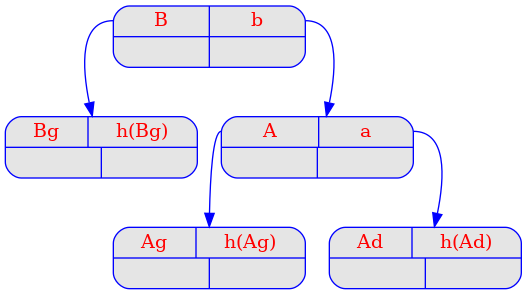
\includegraphics[scale=0.35]{Img_prog1/LeftRotate1.png}
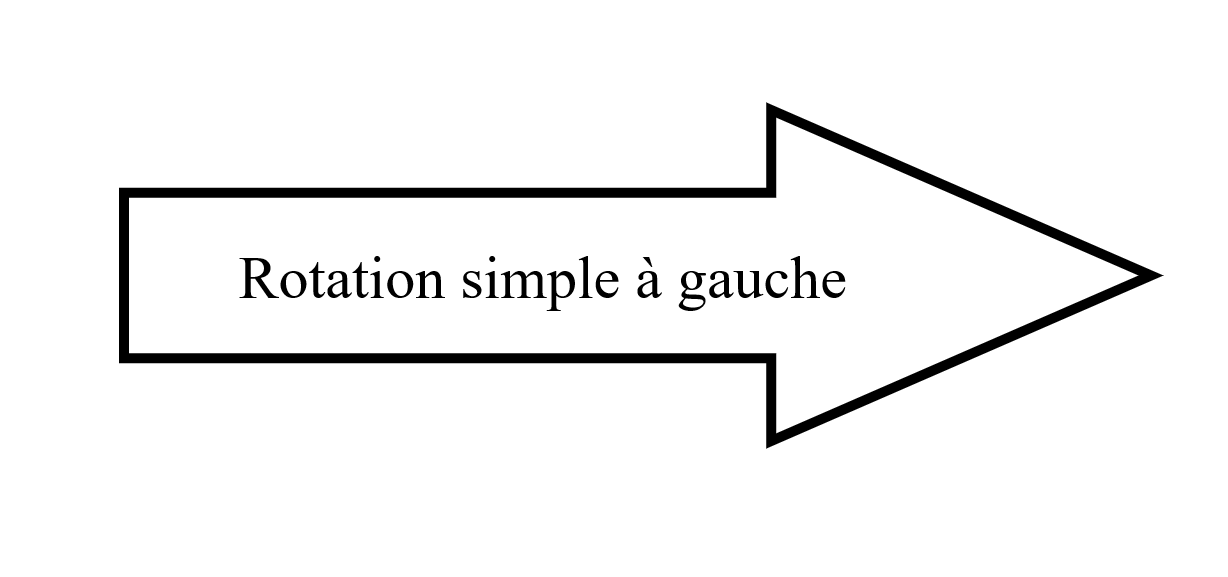
\includegraphics[scale=0.20]{Img_prog1/FlecheLeftrotate.png}
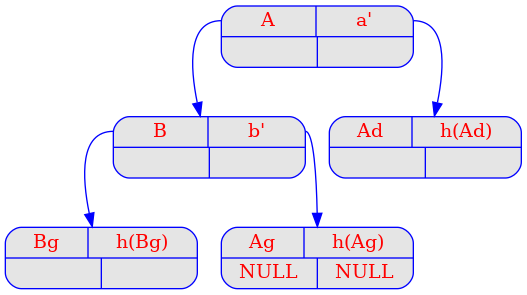
\includegraphics[scale=0.35]{Img_prog1/LeftRotate2.png}
\end{center}

\caption{Rotation simple à gauche}
\label{LeftRot}
\end{figure}

\paragraph{BalanceAVL} Algorithme donné pour la première partie de la fonction, la seconde partie est l'exacte analogie pour un arbre qui penche de l'autre coté. Lors du développement de cette fonction, nous nous sommes heurté à un problème pour les tests afin de savoir l'arbre penche, en effet pour faire une rotation double, il faut que le facteur de déséquilibre soit forcément de 2 en valeur absolue et pas seulement non nul, ie l'arbre est bien déséquilibré. Mais une fois rentré dans la rotation double, pour savoir si on fait une rotation double du même coté, ou des deux cotés différents il suffit que l'arbre penche, ie que le facteur de déséquilibre du second nœud a tourner soit non nul. 


\paragraph{InsertAVL} Algorithme donné donc pas de remarques particulières.

\subsubsection{Lecture du fichier}
En se basant sur \cite{lect_lines}, nous lisons ligne par ligne le fichier, car il y a mot par ligne dans le fichier, en ajoutant un compteur de lignes lues afin de respecter le nombre de mots à mettre dans l'arbre renseigné par l'utilisateur.  

\subsubsection{Affichage avec graphviz}
Les fonctions permettant de générer le fichier \texttt{.dot} étaient déjà données, néanmoins le programme ne prenait en compte les noms composés (ie les noms avec un tiret dedans). Afin de corriger cette erreur, il a fallut ajouter des guillemets (donc la séquence suivant \texttt{\textbackslash "\%s\textbackslash "}) dans les noms des blocs graphviz à afficher. De plus, l'affichage du facteur de déséquilibre n'était pas configuré, nous l'avons donc ajouté à coté du nom de famille du nœud.


\subsection{Jeux de test, exemples d'exécution}
On trouve en figure~\ref{fig:prog1_1} , les différentes étapes de construction de l'arbre pour 10 premiers mots du fichier \texttt{PrenomsV2.txt}. 

\begin{figure}[p]
  
  \begin{center}
    \rule{\linewidth}{.5pt}
    \subcaptionbox{Etape 1}{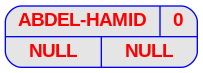
\includegraphics[scale=0.5]{Img_prog1/displayAVL_v00.png}} \vline
    \subcaptionbox{Etape 2}{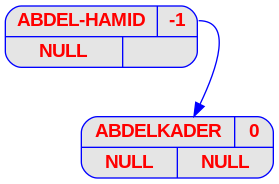
\includegraphics[scale=0.5]{Img_prog1/displayAVL_v01.png}} \vline
    \subcaptionbox{Etape 3}{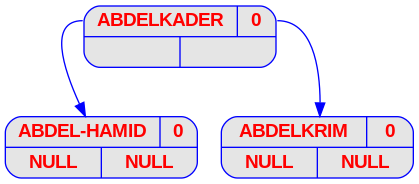
\includegraphics[scale=0.5]{Img_prog1/displayAVL_v02.png}} \rule{\linewidth}{.5pt} %\vline
    \subcaptionbox{Etape 4}{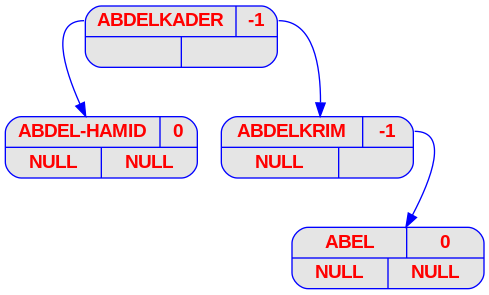
\includegraphics[scale=0.3]{Img_prog1/displayAVL_v03.png}} \vline
    \subcaptionbox{Etape 5}{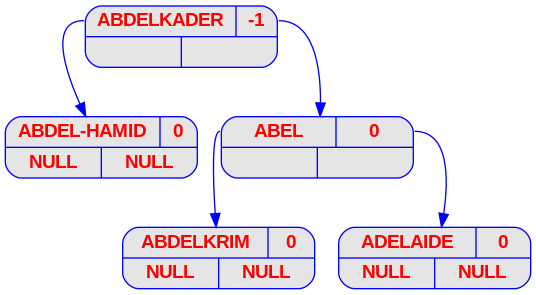
\includegraphics[scale=0.3]{Img_prog1/displayAVL_v04.png}} \vline
    \subcaptionbox{Etape 6}{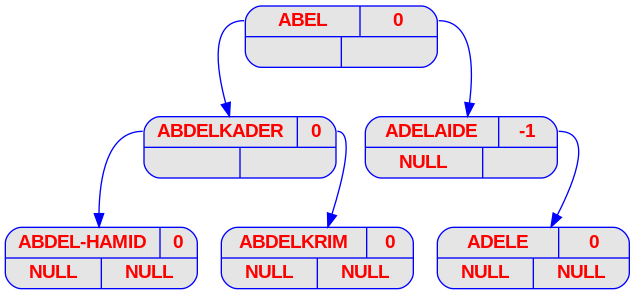
\includegraphics[scale=0.3]{Img_prog1/displayAVL_v05.png}} \rule{\linewidth}{.5pt} %\vline
    \subcaptionbox{Etape 7}{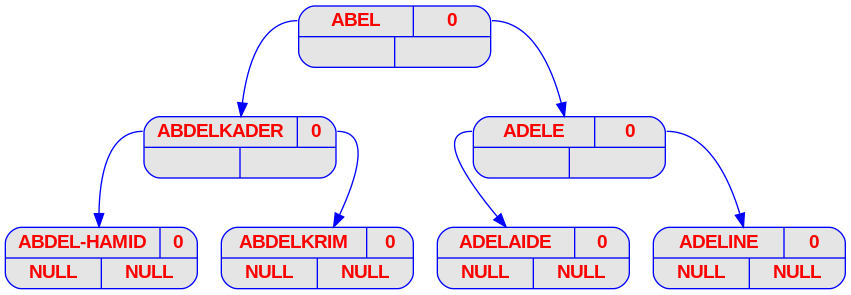
\includegraphics[scale=0.3]{Img_prog1/displayAVL_v06.png}} \vline
    \subcaptionbox{Etape 8}{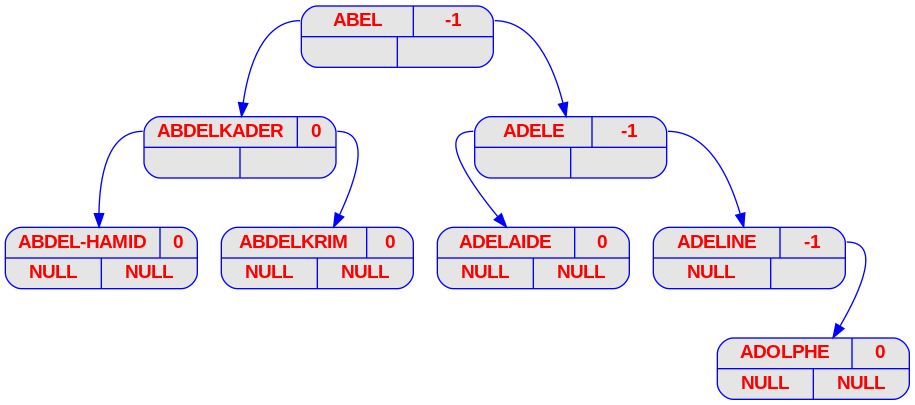
\includegraphics[scale=0.3]{Img_prog1/displayAVL_v07.png}} \rule{\linewidth}{.5pt} %\vline
    \subcaptionbox{Etape 9}{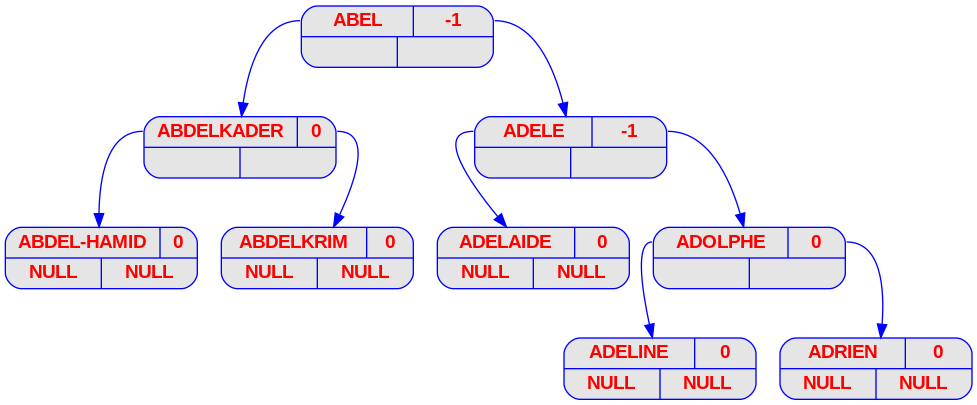
\includegraphics[scale=0.25]{Img_prog1/displayAVL_v08.png}} \vline
    \subcaptionbox{Etape 10}{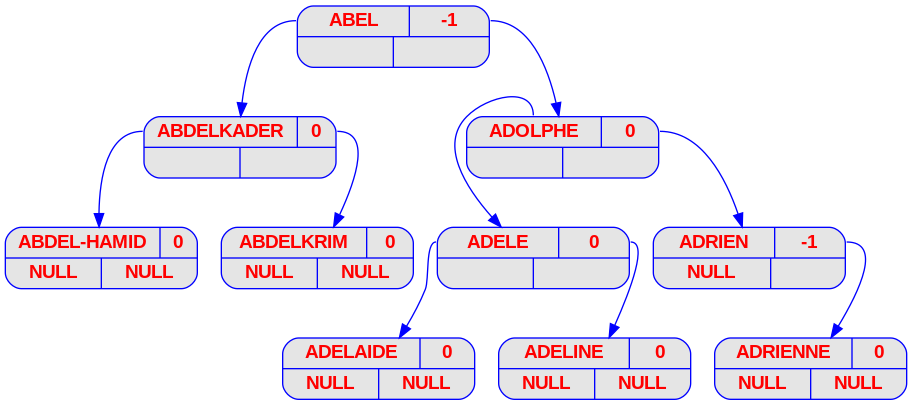
\includegraphics[scale=0.30]{Img_prog1/displayAVL_v09.png}}  \rule{\linewidth}{.5pt} %\vline
   
    
  \end{center}
  
  \caption{Construction de l'arbre pour les 10 premiers prénoms de \texttt{PrenomsV2.txt}}
  \label{fig:prog1_1}
\end{figure}

\begin{figure}[p]
  \begin{center}
    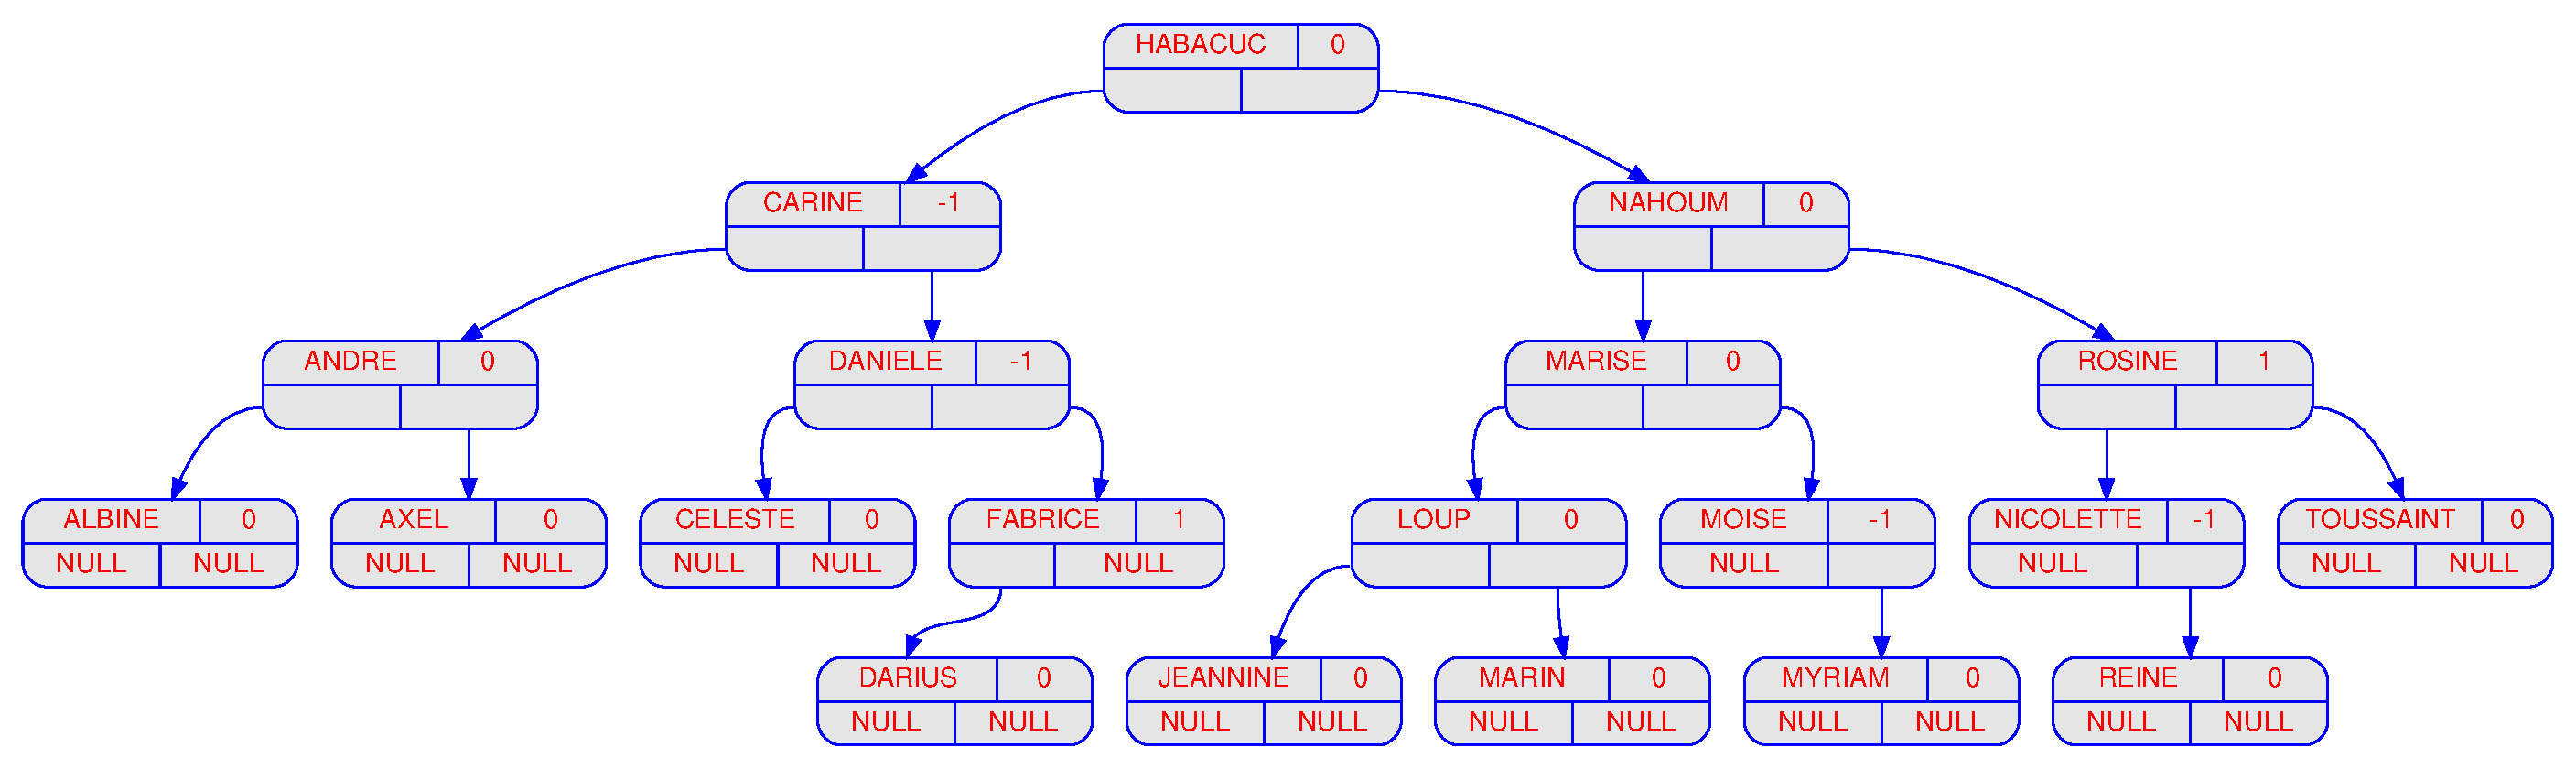
\includegraphics[scale=0.25]{Img_prog1/displayAVL_20.eps}
  \end{center}
  \caption{Example arbre avec les 20 premiers prénoms de \texttt{PrenomsV1.txt}}
\end{figure}

\section{Programme 2: indexation.exe}
\subsection{Développement}


\subsubsection{Fonction de base pour créer l'arbre}
\paragraph{Restructuration des mailles} Pour ce programme, nous avons rajouté un champ dans chaque maille de l'arbre. Dans un premier temps, nous avons décidé que le champ \texttt{T\_avl NodeAVL->val} deviendrai la signature des mots contenus dans le nouveau champ \texttt{T\_avl NodeAVL->list\_mots} qui contient la liste de tout les mots comportant la même signature. Voir illustration des champs d'une maille en figure~\ref{fig:champs_maille} et un exemple en figure~\ref{fig:exemple:maille}.

\begin{figure}[H]
  \begin{center}
    \subcaptionbox{Champs de la maille\label{fig:champs_maille}}{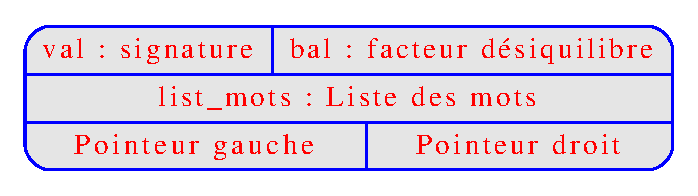
\includegraphics[scale=0.75]{Img_prog2/Maille_vide.eps}}
    \subcaptionbox{Exemple de maille\label{fig:exemple:maille}}{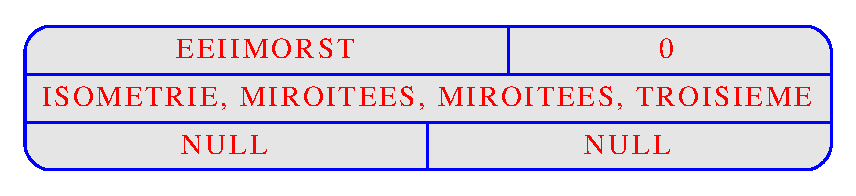
\includegraphics[scale=0.75]{Img_prog2/Maille_exemple.eps}}
  \end{center}
  \caption{Restructuration des mailles pour le second programme}
  \label{fig:restruc_pro2}
\end{figure}

\paragraph{Ajout dans les mailles}
\subsubsection{Calcul des paramètres de l'arbre}
\subsubsection{Recherche de mots}

\subsection{Jeux de test, exemples d'exécution}



\section{Programme 3: anagrammes.exe}
\subsection{Développement}
\subsection{Jeux de test, exemples d'exécution}



\section{Gestion de projet}
\section{Conclusion}



\nocite{*}

\bibliography{bibli}
\bibliographystyle{plain}


\end{document}